\chapter{The multi-dimensional case} \label{chap5}

In this last chapter we are going to examine a more complex situation. We now want to model the movement of a particle in $\R^{n}$ with periodically distributed, smooth, $n-1$-dimensional surfaces inducing a potential. The basic concept of the previous chapters can be easily extrapolated to this multidimensional case, and therefore the main result remains the same. Consequently, the proves basically do not differ from the one-dimensional case and hence most of the subsequent theorems will be merely argumentatively justified.
~\newline ~\newline
For this, let $Y$ denote a periodicity cell in $\R^{n}$ and $B^{n}$ the corresponding Brillouin zone, for simplicity assume $Y$ being the unit cube $Y = [0, 1]^{n}$ and hence $B = [-\pi, \pi]^{n}$. Contained in $Y$ let $S$ be a smooth surface, without a boundary with the conditions $\dim S = n - 1$ and $S \subseteq \overset{\circ}{Y}$. Furthermore, let $B \subseteq Y$ denote the set enclosed by $S$, such that $S = \partial B$. We will denote for any $j \in \Z^{n}$ with $Y_{j} = Y + j$ the $j$th copy of $Y$, which results through translation of the periodicity cell by $j$, and analogously for $S_{j} = S + j$ and $B_{j} = B + j$. % todo some better explanations

\begin{figure*}[h!] \centering
	  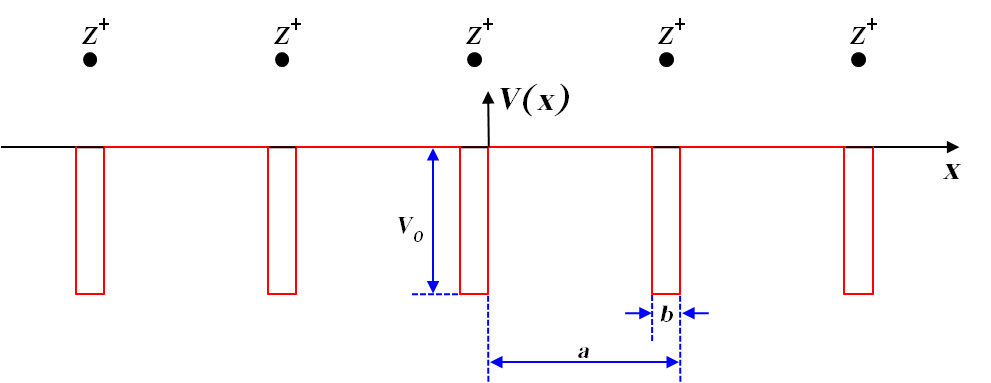
\includegraphics[width=0.75\textwidth]{Periodic_square_potential_130707} 
\end{figure*}
~\newpage % todo temporarily
The mathematical representation of the above is a multi-dimensional Schrödinger operator $A^{n}$ whose operation is formally defined by
\begin{equation}
	- \Delta + \rho \sum_{i \in \Z} \delta_{S_{i}} \label{the-operator-A-formally}
\end{equation}
on the whole of $\R^{n}$, where $\delta_{S_{i}}$ denotes the Dirac delta distribution on hypersurface $S_{i}$, that integrates any function $u \in L^{2}(\R)$ over the compact set $S_{i}$
~\\ ~\\ 
Again motivated by the weak-formulation, given a right-hand side $f \in L^{2}(\R^{n})$ we consider for some $\mu \in \R$ the problem to find $u \in H^{1}(\R^{n})$ such that
	\begin{equation}
		\int_{\R^{n}} \nabla u \overline{\nabla v} + \rho \sum_{i \in \Z^{n}} \int_{S_{j}} u \overline{v} ds - \mu \int_{\R^{n}} u \overline{v} = \int_{Y} f \overline{v} \label{md-weak-formulation}
	\end{equation} 
holds for all $v \in H^{1}(\R^{n})$, where $s$ is the hypersurface measure associated to all $S_{j}$ \cite. 

\begin{remark}
	The term originating from the potential is finite as
	\[ \left| \sum_{j \in \Z^{n}} \int_{S_{j}} u \overline{v} \right|^{2} \leq \left( \sum_{j \in \Z^{n}} \| u \|_{L^{2}(S_{j})}^{2} \right) \left( \sum_{j \in \Z^{n}} \| v \|_{L^{2}(S_{j})}^{2} \right). \]
	Both terms on the right-hand side can be finitely estimated by the Trace theorem \cite[Chap. 5]{Evans98} as
	\[ \| u \|_{L^{2}(S_{j})}^{2} \leq 2 \left( \frac{1}{h} \|u\|_{L^{2}(B_{j})}^{2} + h \| \nabla u \|_{L^{2}(B_{j})}^{2} \right) \]
	for some $h > 0$. % todo more explicite
\end{remark}

We can once again exert Lax-Migram's Theorem to prove in \eqref{md-weak-formulation} the existence of a unique solution $u \in H^{1}(\R^{n})$ in \eqref{md-weak-formulation} for any $f \in L^{2}(\R^{n})$ if $\mu$ is small enough, define the operator injective $R_{\mu}^{n} \colon f \mapsto u$ and define $A$ by means of $R_{\mu}^{n}$.

\begin{remark}
	The operator $A$ is self-adjoint.	
\end{remark}


\begin{theorem}[Characterisation of $\mathcal{D}(A)$] Let $\Omega \coloneqq \R^{n} \setminus \overline{\bigcup_{j \in \Z^{n}} B_{j}}$. By choosing similar to above different functions $v \in C^{\infty}(\R^{n})$ in \eqref{md-weak-formulation} we can further characterise such $u \in \mathcal{D}(A)$, namely for all $j \in \Z^{n}$ it holds:
	\begin{enumerate}
		\item $\Delta u \in L^{2}(B_{j})$, $\Delta u \in L^{2}(\Omega)$ and $\sum_{j \in \Z^{n}} \|\Delta u \|_{L^{2}(B_{j})}^{2} < \infty$
		\item $u \big|_{S_{j} - 0} = u \big|_{S_{j} + 0}$
		\item $\frac{\partial u}{\partial \eta_{j}} \big|_{S_{j} - 0} - \frac{\partial u}{\partial \eta_{j}} \big|_{S_{j} + 0} - \rho u \big|_{S_{j}} = 0$ where $\eta_{j}$ denotes the normal on $S_{j}$
	\end{enumerate}
\end{theorem}

Now, restricting again this problem to a fundamental domain of periodicity, for example $Y$,
\begin{figure*}[h!] \centering
	  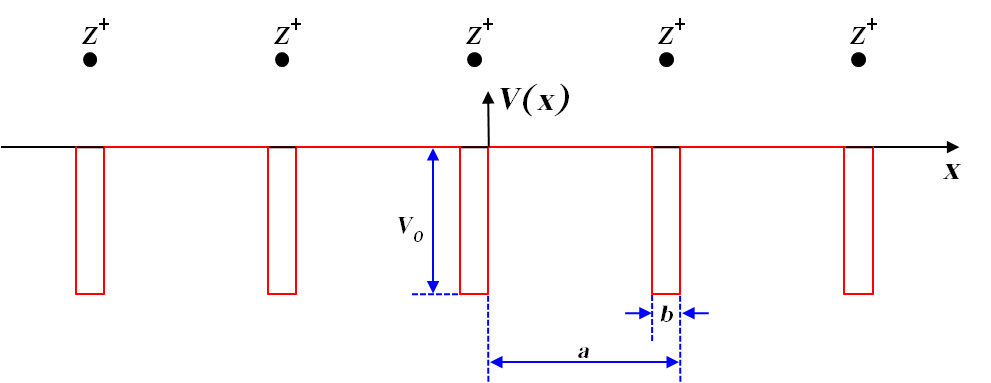
\includegraphics[width=0.75\textwidth]{Periodic_square_potential_130707} 
\end{figure*}

yields an operator $A^{n}_{k}$ which we can define by proceeding as previous with the problem to find $u \in H^{1}_{k, n} \coloneqq \big\{ w \in H^{1}(Y) \colon w \big|_{S_{j}^{+}} = w \big|_{S_{j}^{+}} e^{i k_{j}}$ for $k \in [-\pi, \pi]^{2}, j = 1,2 \big\}$ such that
	\begin{equation}
		\int_{Y} \nabla u \overline{\nabla v} + \rho \int_{S} u \overline{v} ds - \mu \int_{Y} u \overline{v} = \int_{Y} f \overline{v}. \label{md-weak-formulation-res}
	\end{equation} 
for for all $v \in H^{1}_{k, n}$.
~\newline ~\newline
Again, Lax-Milgram's Theorem ensures the existence of a unique solution $u \in H^{1}_{k, n}$ if $\mu$ is small enough, and the operator $R_{\mu, k} \colon f \mapsto u$ is well-define and injective. In return we are able to define 
	\[ A_{k}^{n} \coloneqq R_{\mu, k}^{n} + \mu I \]
It is easy to see that such a solution $u \in H^{1}_{k, n}$ has to satisfy even more, especially:
	\[ \frac{\partial u}{\partial x_{j}}\big|_{S_{j}^{+}} = e^{ik_{j}} \frac{\partial u}{\partial x_{j}}\big|_{S_{j}^{-}} \quad j = 1,2  \]
	
\begin{theorem}
	The operator $R_{\mu, k}^{n}$ on the fundamental domain of periodicity is compact.	

	\begin{proof}
		Analogous to , for the compact embedding see \cite[Chap. 4]{Adams}.	
	\end{proof}
\end{theorem}

By similar transformations of the problem \eqref{md-weak-formulation-res} as in \eqref{mod-eigv-problem} and \eqref{periodic-condition} we are able to show that the eigenvalues of $A^{n}_{k}$ are continuous functions of $k \in \overline{B}$, and thus $I_{s} = \{ \lambda_{s}(k) : k \in \overline{B} \}$ is a compact real interval for each $s \in \N$.
~\newline ~\newline
Ultimately, using the same arguments as in Chapter 4 through Bloch waves, Floquet transform and a similar cut-off function $\eta$ as in \eqref{eta} we are able to prove the main result even for this multi-dimensional case, namely that the spectrum of a self-adjoint Schrödinger operator with periodic delta-potential on a hypersurface is the union of compact intervals, i.e.
	\[ \sigma(A) = \bigcup_{s \in \N} I_{s}. \]
We have to notice that we haven't determined the nature of the spectrum that is if there are possible gaps in the spectrum. However,... % todo schluss